\documentclass{article}
\usepackage[utf8]{inputenc}
\usepackage[russian]{babel}
\usepackage[left=2cm,right=2cm,
top=2cm,bottom=2cm,bindingoffset=0cm]{geometry}
\usepackage{graphicx}
\usepackage{amsmath}
\usepackage{float}
\usepackage{listings}
\usepackage{url,textcomp}
\date{2019 г.}
\author{Кондратенко Федор, гр 13632/1}
\setlength{\parindent}{0pt}
\setlength{\parskip}{5pt plus 2pt minus 1pt}
\frenchspacing
\title{Отчет по заданию №2.1}
\begin{document}
	\maketitle
	\section*{Модель}
	В качестве исходной была взята модель из задания 3.1. В нее был внесен ряд изменений, а именно:
	\begin{enumerate}
		\item Вместо коэффициента $b$ задается коэффициент $\psi$;
		\item Проведен рефакторинг системы, создана вспомогательная подсистема подсистемы для расчета коэффициентов;
		\item Добавлены блоки анализа системы.
	\end{enumerate}
	Внешний вид модели:
	\begin{figure}[H]
		\centering
		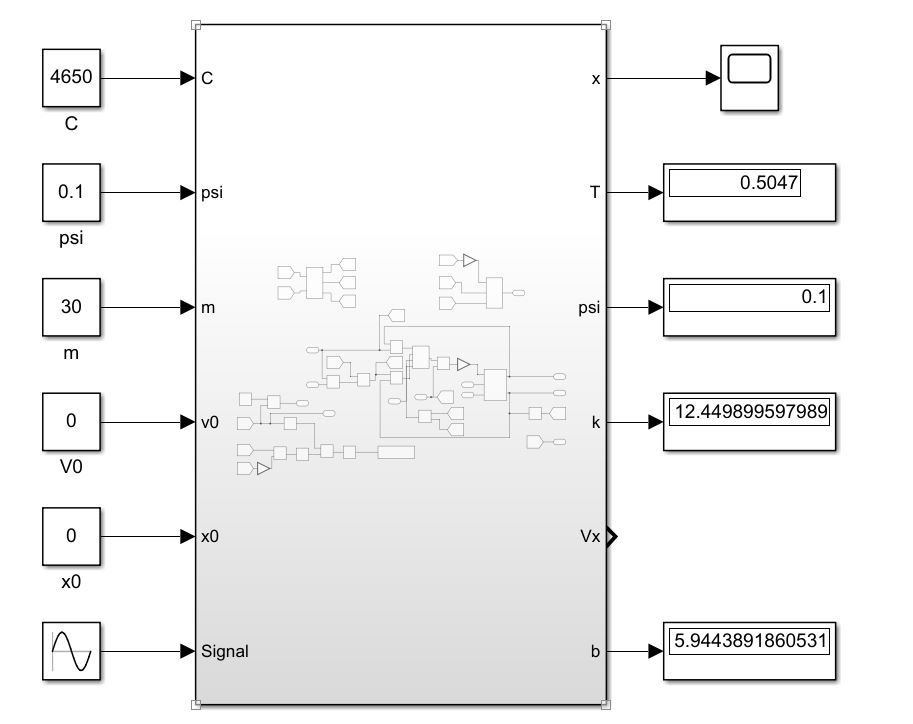
\includegraphics[width=0.7\linewidth]{model_outdoor}
		\caption{Внешний вид модели}
		\label{fig:modeloutdoor}
	\end{figure}
	Подсисистема:
	\begin{figure}[H]
		\centering
		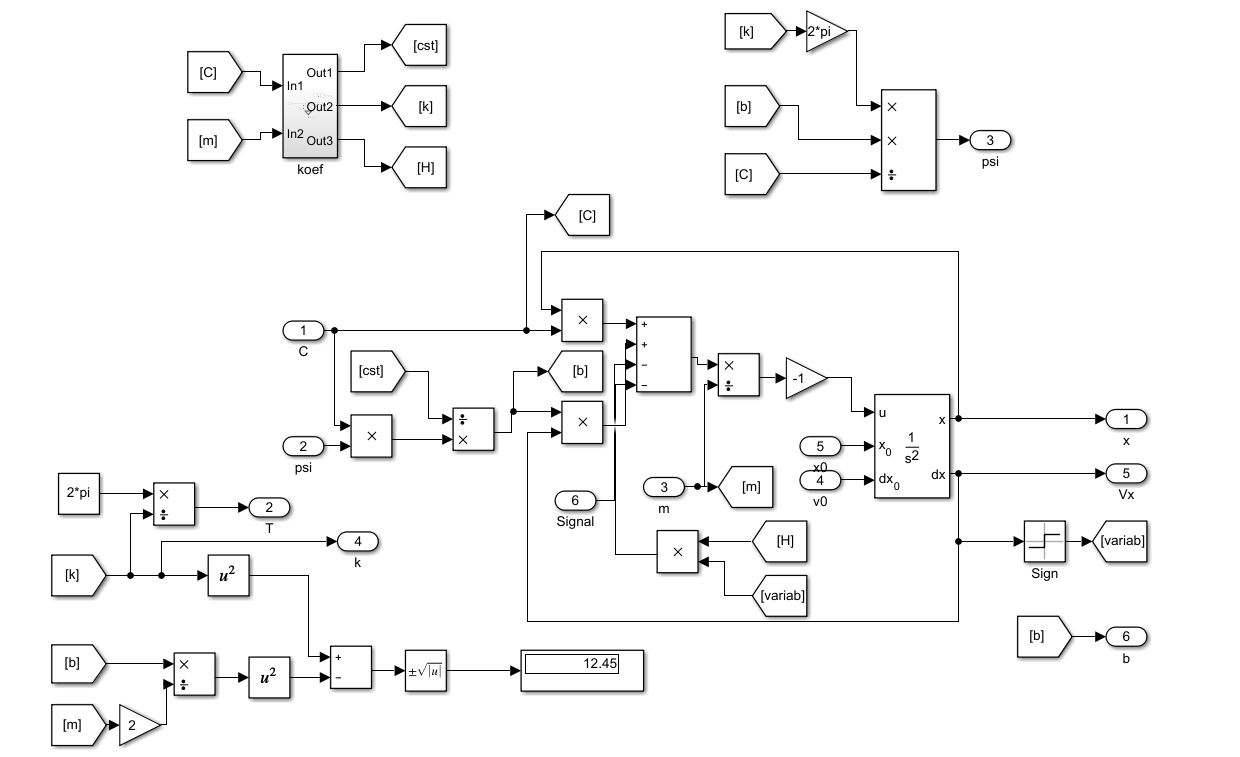
\includegraphics[width=1.1\linewidth]{model_all}
		\caption{Вид подсистемы}
		\label{fig:modelall}
	\end{figure}
	Дифференциальные уравнения колебаний остались теми же, за исключением уравнения для последнего задания.
	Вспомогательная подсистема:
	\begin{figure}[H]
		\centering
		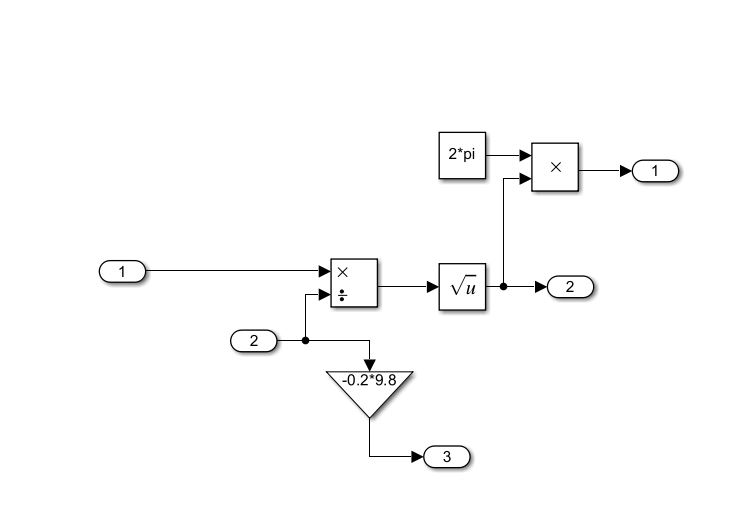
\includegraphics[width=0.7\linewidth]{koef}
		\caption{Вспомогательная подсистема. Вычисляет некоторые коэффициенты, которые далее используются при моделировании.}
		\label{fig:koef}
	\end{figure}
	\section*{Результаты моделирования и анализ системы}
	\begin{figure}[H]
		\centering
		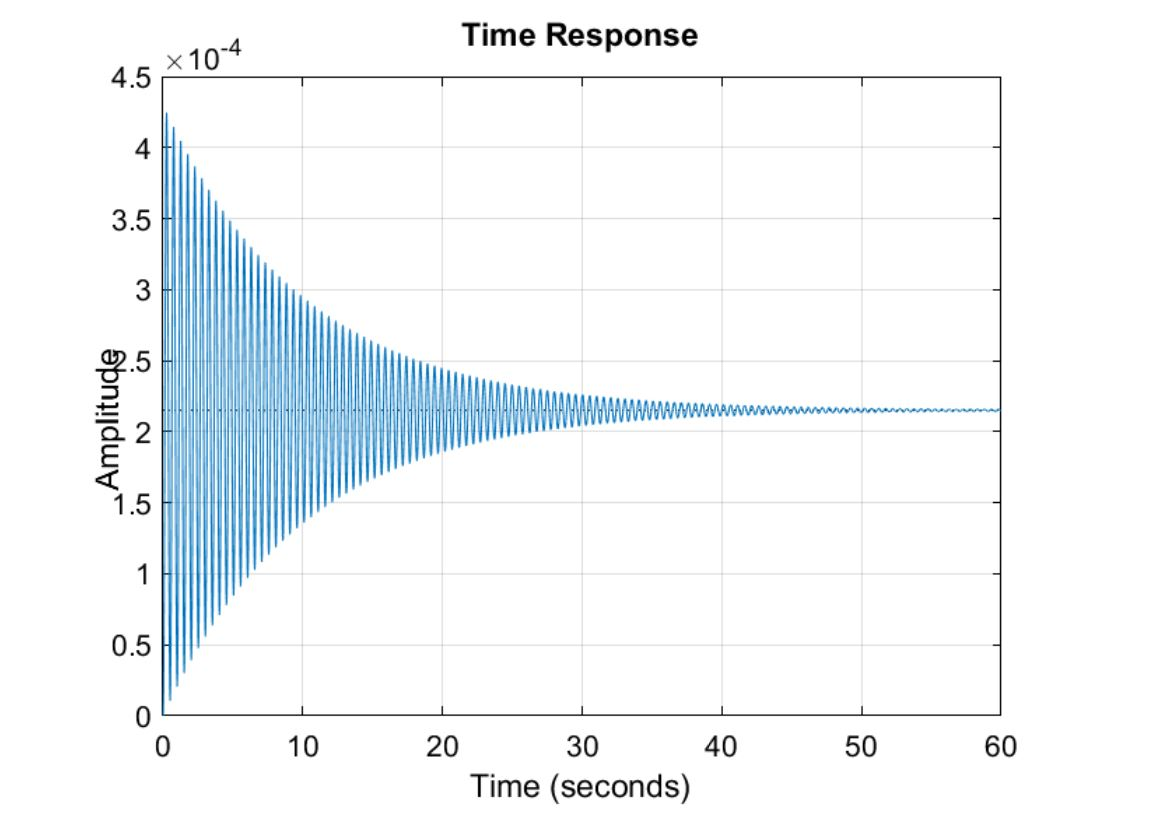
\includegraphics[width=0.7\linewidth]{graph1}
		\caption{Linear step response plot, $\psi$=0.1}
		\label{fig:graph1}
	\end{figure}
	
\end{document}